\apendice{Planificación}

\section{Introducción}


Para llevar a cabo este proyecto vamos a aplicar una metodología llamada Scrum. Scrum es una metodología de desarrollo software ágil, es decir, durante cada \textit{sprint} \footnote{\textit{Sprint}: es el período en el cual se lleva a cabo el trabajo en sí.\cite{wiki:scrum}} se asignarán unas determinadas tareas a cumplimentar, con un producto como consecuencia de estas tareas. Al final de cada \textit{sprint} se realizará una reunión junto a los tutores para validar los avances realizados y determinar las tareas a realizar durante el siguiente \textit{sprint}.

% \section{Estudio previo}

\subsection{\textit{Sprint} 0}
Estas son las tareas a realizar durante este \textit{sprint} 0:

\begin{itemize}
	\item Probar \LaTeX.
	\item Gestor de tareas/versiones: \textit{Github} y \textit{Zenhub}.
	\item Instalar \textit{Anaconda} y \textit{Jupyter}.
	\item Leer los artículos propuestos por los tutores.
	\item Comenzar a probar algunos algoritmos de binarización.
\end{itemize}

Como se puede ver las tareas a realizar son básicas, puesto que es el \textit{sprint} 0 y es un \textit{sprint} de mera adaptación al entorno de trabajo. La única tarea que supone un esfuerzo de comprensión mayor es la lectura de los artículos propuestos sobre trabajos relacionados o con una problemática similar a la nuestra. A continuación, en la figura \ref{fig:A.1.1}, se muestra el diagrama \textit{burndown} de este \textit{sprint}. 

\begin{figure}[h]
\centering
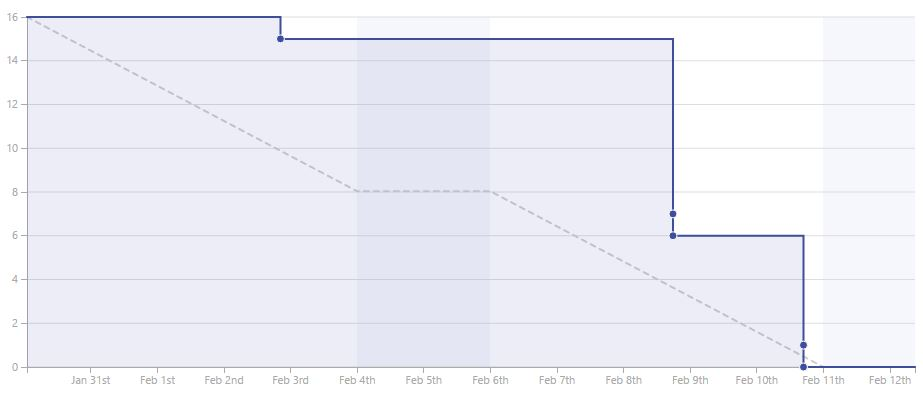
\includegraphics[width=0.99\textwidth]{sprint_0}
\caption{Burndown del \textit{sprint} 0}
\label{fig:A.1.1}
\end{figure}

\subsection{\textit{Sprint} 1}
Estas son las tareas a realizar durante esta \textit{sprint} 1:

\begin{itemize}
	\item Documentar lo realizado durante el \textit{sprint} 0.
	\item Documentar lo que se irá realizando durante este \textit{sprint} 1.
	\item Continuar probando con algoritmos de procesamiento de imágenes.
	\item Probar una aproximación con clasificadores al problema.
\end{itemize}

Puesto que en el \textit{sprint} anterior no se documentó lo realizado, durante este se pretende documentar todo lo realizado durante el \textit{sprint} anterior y este. Además de continuar probando con algoritmos de procesamiento de imágenes y comenzar a probar con la aproximación al problema mediante clasificadores.

En este \textit{sprint} me vi desbordado de trabajo debido a la subestimación del esfuerzo a empeñar en las distintas tareas. No siendo capaz de comenzar a probar una aproximación con clasificadores. Por ello la tarea <<Probar una aproximación con clasificadores al problema>> se vio movida al siguiente \textit{sprint}. 

A continuación, en la figura \ref{fig:A.1.2}, se muestra el diagrama \textit{burndown} de este \textit{sprint}. El cual tiene dicho aspecto debido a que muchas de las tareas se trabajaron de manera paralela, no siendo acabadas hasta el final del \textit{sprint}. Y, además, algunas de las tareas no fueron cerradas cuando se debió, aspecto que se corregirá en los siguientes \textit{sprints}.

\begin{figure}[h]
\centering
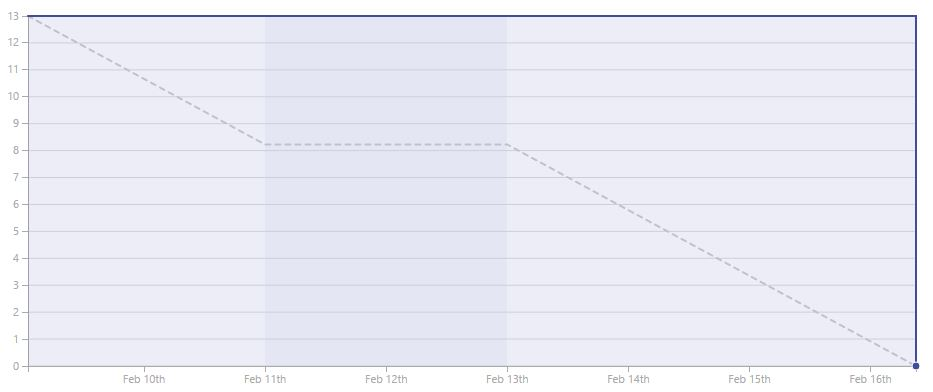
\includegraphics[width=0.99\textwidth]{sprint_1}
\caption{Burndown del \textit{sprint} 1}
\label{fig:A.1.2}
\end{figure}

\subsection{\textit{Sprint} 2}
Estas son las tareas a realizar durante este \textit{sprint} 2:

\begin{itemize}
	\item Probar una aproximación con clasificadores al problema.
	\item Aplicación del método "Non maximum suppression" sobre el clasificado.
\end{itemize}

Puesto que la aproximación mediante reconocimiento de imágenes no reflejaba unos resultados muy positivos, durante la reunión mantenida con los tutores se decidió el uso de una técnica distinta. Nos referimos a la utilización  de un clasificador, junto a un descriptor visual.

Debido a que todavía no se poseían suficientes imágenes para el estudio del problema mediante esta técnica, lo que se decidió es aplicarla sobre otro problema de características similares, como es el reconocimiento de caras en imágenes. Con unos resultados bastante positivos debido a distintos razonamientos explicados en la Memoria, sección de Aspectos relevantes del proyecto.

A continuación, en la figura \ref{fig:A.1.3}, se muestra el diagrama \textit{burndown} de este \textit{sprint}.

\begin{figure}[h]
\centering
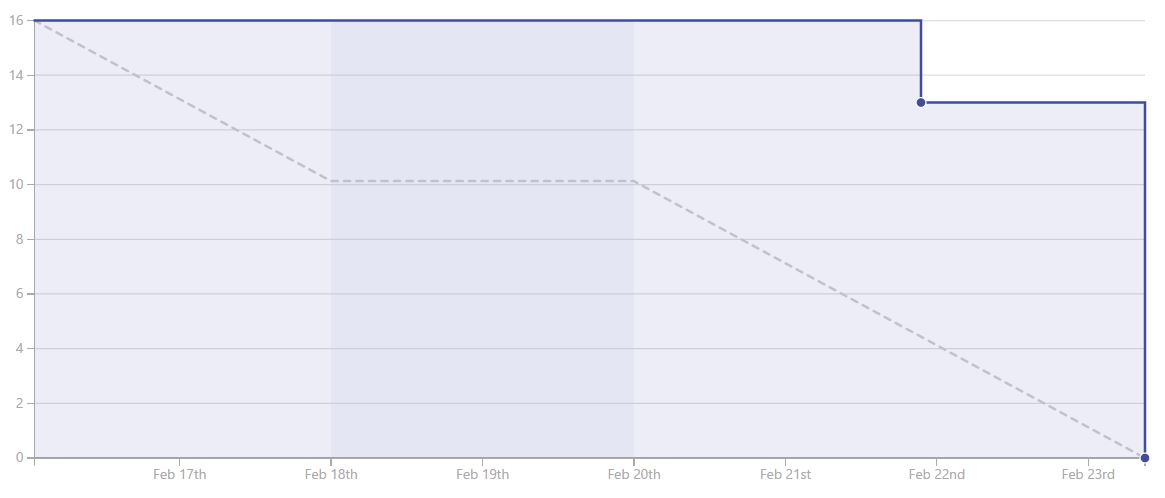
\includegraphics[width=0.99\textwidth]{sprint_2}
\caption{Burndown del \textit{sprint} 2}
\label{fig:A.1.3}
\end{figure}

\subsection{\textit{Sprint} 3}
Estas son las tareas a realizar durante este \textit{sprint} 3:

\begin{itemize}
	\item Reorganizar los \textit{Jupyter Notebooks}.
	\item Probar distintos clasificadores y métricas.
	\item Enviar fotos rotadas al clasificador.
\end{itemize}

Durante este \textit{sprint}, primero, se reorganizo la estructura del proyecto. Aportando mucho más orden y claridad a nuestro proyecto. Después, se introdujeron múltiples clasificadores y métricas, los cuales introduciré en mayor medida en la memoria, como \textit{Random Forest} o \textit{Gradient tree boosting}. Por último, se enviaron imágenes rotadas al clasificador, con el fin de poder analizar una posible problemática.

A continuación, en la figura \ref{fig:A.1.4}, se muestra el diagrama \textit{burndown} de este \textit{sprint}.

\begin{figure}[h]
\centering
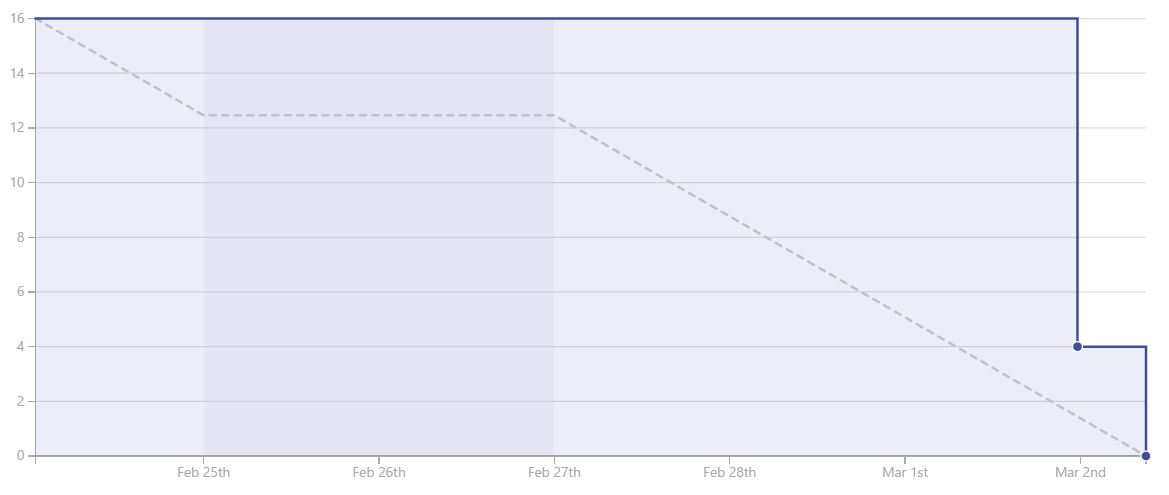
\includegraphics[width=0.99\textwidth]{sprint_3}
\caption{Burndown del \textit{sprint} 3}
\label{fig:A.1.4}
\end{figure}

\subsection{\textit{Sprint} 4}
Estas son las tareas a realizar durante este \textit{sprint} 4:

\begin{itemize}
	\item Implementación de \textit{Data Augmentation} en nuestro conjunto de entrenamiento.
	\item Implementación de controles de usuario.
\end{itemize}

Durante este \textit{sprint} se aplicó en nuestro conjunto de entrenamiento la técnica \textit{Data augmentation}. Esta técnica nos permitió aumentar el tamaño de nuestro conjunto de entrenamiento enormemente. 

Además, se realizó un \textit{notebook}\footnote{Siempre que nos referimos a un \textit{notebook}, a lo que nos referimos es a un \textit{Jupyter Notebook}}, con controles de usuario, los cuales nos permiten escoger entre clasificadores, imágenes y probabilidades. Permitiendo la continua interacción entre el usuario y la clasificación de una imagen, sin la necesidad de modificar el código por parte del usuario del notebook para cambiar entre las distintas opciones.

A continuación, en la figura \ref{fig:A.1.5}, se muestra el diagrama \textit{burndown} de este \textit{sprint}.

\begin{figure}[h]
\centering
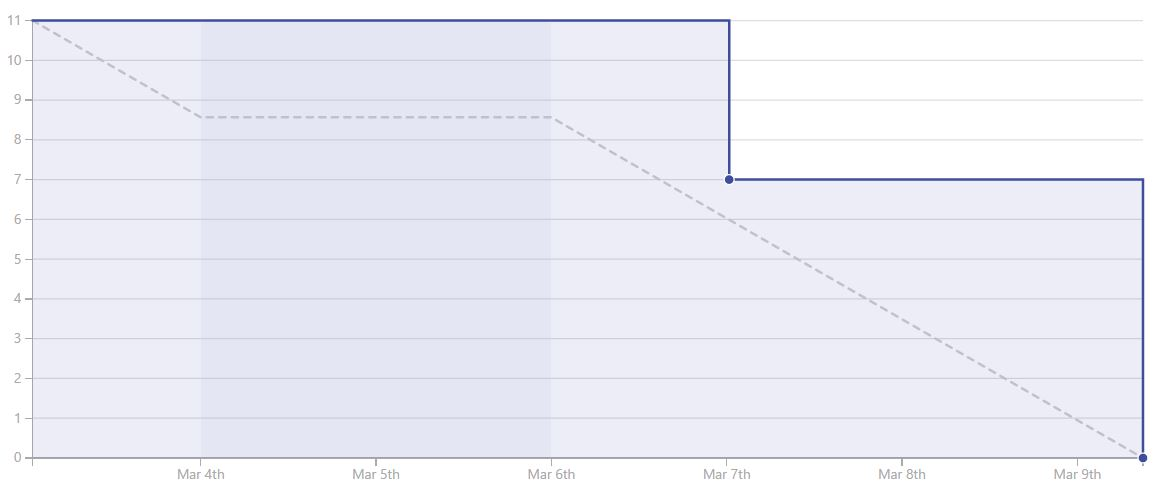
\includegraphics[width=0.99\textwidth]{sprint_4}
\caption{Burndown del \textit{sprint} 4}
\label{fig:A.1.5}
\end{figure}


\subsection{\textit{Sprint} 5}
Estas son las tareas a realizar durante este \textit{sprint} 4:

\begin{itemize}
	\item Implementar un \textit{file chooser} 
	\item Añadir más clasificadores.
	\item Correciones en la documentación.
	\item Estudiar como implementar un etiquetador de imágenes.
\end{itemize}


\begin{comment}
\begin{figure}[h]
\centering
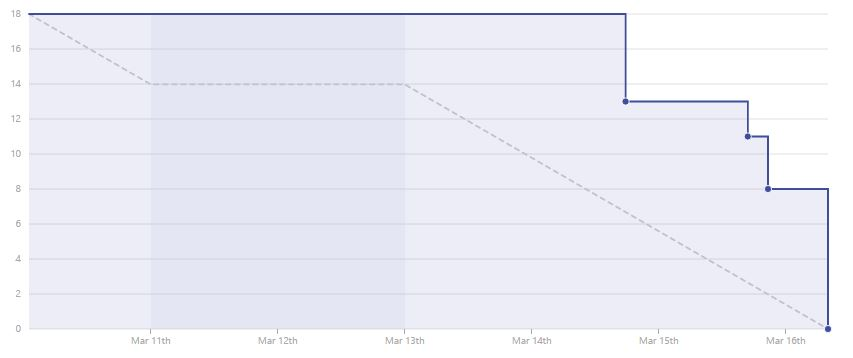
\includegraphics[width=0.99\textwidth]{sprint_5}
\caption{Burndown del \textit{sprint} 5}
\label{fig:A.1.5}
\end{figure}
\end{comment}

\section{Planificación temporal}

\section{Estudio de viabilidad}

\subsection{Viabilidad económica}

\subsection{Viabilidad legal}


